\begin{document}
%=================================================================
%                           Start Document
%=================================================================
\section{Bakgrunn - Teoretisk Grunnlag}


\lhead{Bakgrunn - Teoretisk Grunnlag} % section header

\setstretch{1.6}

\subsection{Functional Electrical Stimulation}
Functional Electrical stimulation (FES) is the application of electrical current to excitable tissue to supplement or replace a function that is lost in neurologically impaired individuals. FES can be used for chronic applications for restoration of function or in therapeutic applications as it is used in the project. The aim of therapeutic electrical stimulation is to improve tissue health or voluntary function by inducing physiological changes that remain after the stimulation. 

Stimulation is delivered as a waveform of electrical current pulses, which are characterized by three parameters: pulse frequency, amplitude and duration, as well as the shape of the pulse train. The strength of the muscle contraction is determined by modulating these parameters.

\begin{figure} [H]
    \centering
    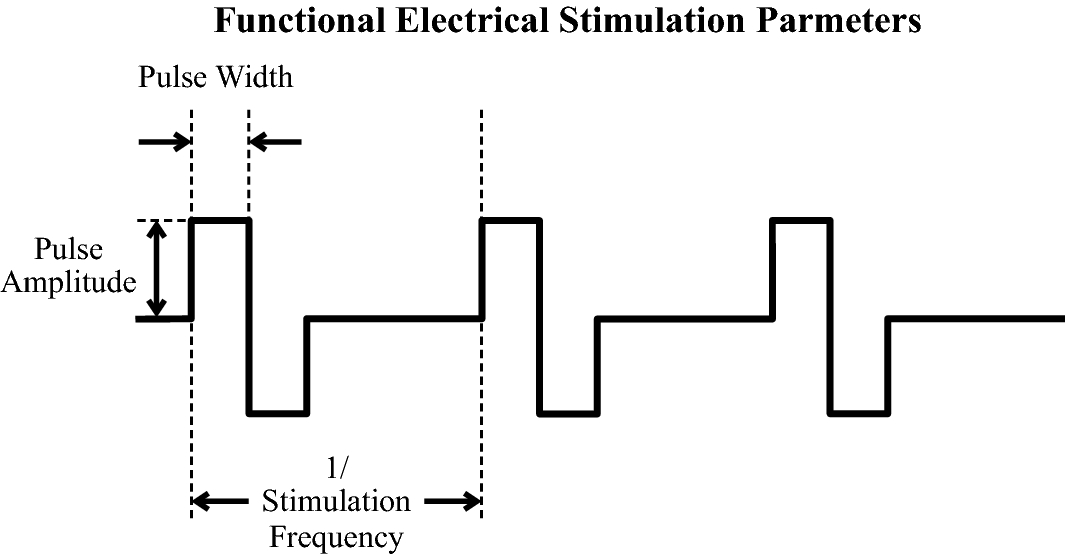
\includegraphics[width=0.7\linewidth]{images/stimpar.png}
    \caption{Illustration of a typical biphasic stimulation waveform and its parameters \cite{marquez-chin_functional_2020}}
    \label{fig:waveforms}
\end{figure}

The resulting torque about the joint that is actuated by the muscle depends on the tension in the flexor and extensor muscles as well as the biomechanics of the joint \cite{lynch_functional_2008}. 

\subsubsection{Limitations}
FES recruits motor units in a synchronous manner, unlike an intact nervous system that recruits in an asynchronously. Thus FES requires a much higher stimulation frequncy (20-40Hz), compared to the typical nervous system frequency (6-8Hz) in order to achieve sustained muscle contraction \cite{lynch_functional_2008}. This is the main cause of the increased rate of fatigue associated with FES contraction as compared to contraction initiated by the central nervous system (CNS) \cite{gilman_handbook_1983}. 

Furthermore FES is believed to recruit the fast-twitch fibers before the slow-twitch fibers, due to the larger diameter of innervation axons. This non-physiological recruitment is the opposite of natural muscle-fiber recruitment order.Since fast-twitch fibers fatigue more quickly than slow twitch fibers, this also leads to the increased fatigue seen with artificial stimulation. \cite{lynch_functional_2008}

When an artificially stimulated muscle begins to fatigue, its response changes non-linearly \cite{lynch_functional_2008}, and will eventually stop contracting. 

FES applications for motor function uses the fundemental principle that electrical stimulation generally activates nerve rather than muscle \cite{peckham_functional_2005}. This is because the threshold charge for directly eliciting muscle fiber action potentials is much gereater than the threshold of producing action potentials in neurons. Thus for FES to be effective, the lower motor neurons must be intact from the anterior horns of the spinal cord to the neuromuscular junctions in the muscles that , as is usually the case with spinal cord injury, stroke, head injuries, cerebral palsy and multiple sclerosis \cite{gregory_recruitment_2005}. 




%=================================================================
%                           End Document
%=================================================================
\end{document}